\documentclass{beamer}

\usepackage{amsmath,amsthm, amssymb, latexsym}
\usepackage{subcaption}
\usepackage[normalem]{ulem}

% Theme stuff
\usetheme{Madrid}

\useinnertheme{circles}

% Define colors
\definecolor{color0}{RGB}{0,0,0} % black, for text
\definecolor{color1}{RGB}{128,0,0} % maroon, for titles, blocks
\definecolor{color2}{RGB}{118,118,118} % dark grey, for blocks
\definecolor{color3}{RGB}{255,253,250} % background color, white
\definecolor{color4}{RGB}{214,214,206} % light grey, title backgrounds
% Set colors for basic beamer elements
\setbeamercolor{headline}{bg=color4}
\setbeamercolor{footline}{bg=color4}
\setbeamercolor{block title}{bg=color4,fg=color1}
\setbeamercolor{frametitle}{bg=color4,fg=color1}
\setbeamercolor{title}{bg=color4,fg=color1}

\colorlet{beamer@blendedblue}{color1}

\newcommand{\T}{\frac{\theta}{2}}
\newcommand{\E}{\mathrm{E}}
\newcommand{\Var}{\mathrm{Var}}
\newcommand{\Cov}{\mathrm{Cov}}
\newcommand{\Pro}{\mathrm{P}}

%% \AtBeginSection[]
%% {
%%   \begin{frame}
%%     \frametitle{Table of Contents}
%%     \tableofcontents[currentsection]
%%   \end{frame}
%% }

\title[quant gen coal]{A neutral model for quantitative trait
  distributions from a coalescent perspective}
\author{Evan Koch}
\date{August 5, 2017}

\begin{document}
\frame{\titlepage}
% \frame{\tableofcontents}

\section{Introduction}

% \subsection{Various models of neutral trait evolution}

\begin{frame}{The factors affecting trait distributions}
  \framesubtitle{Population structure}
  \begin{center}
    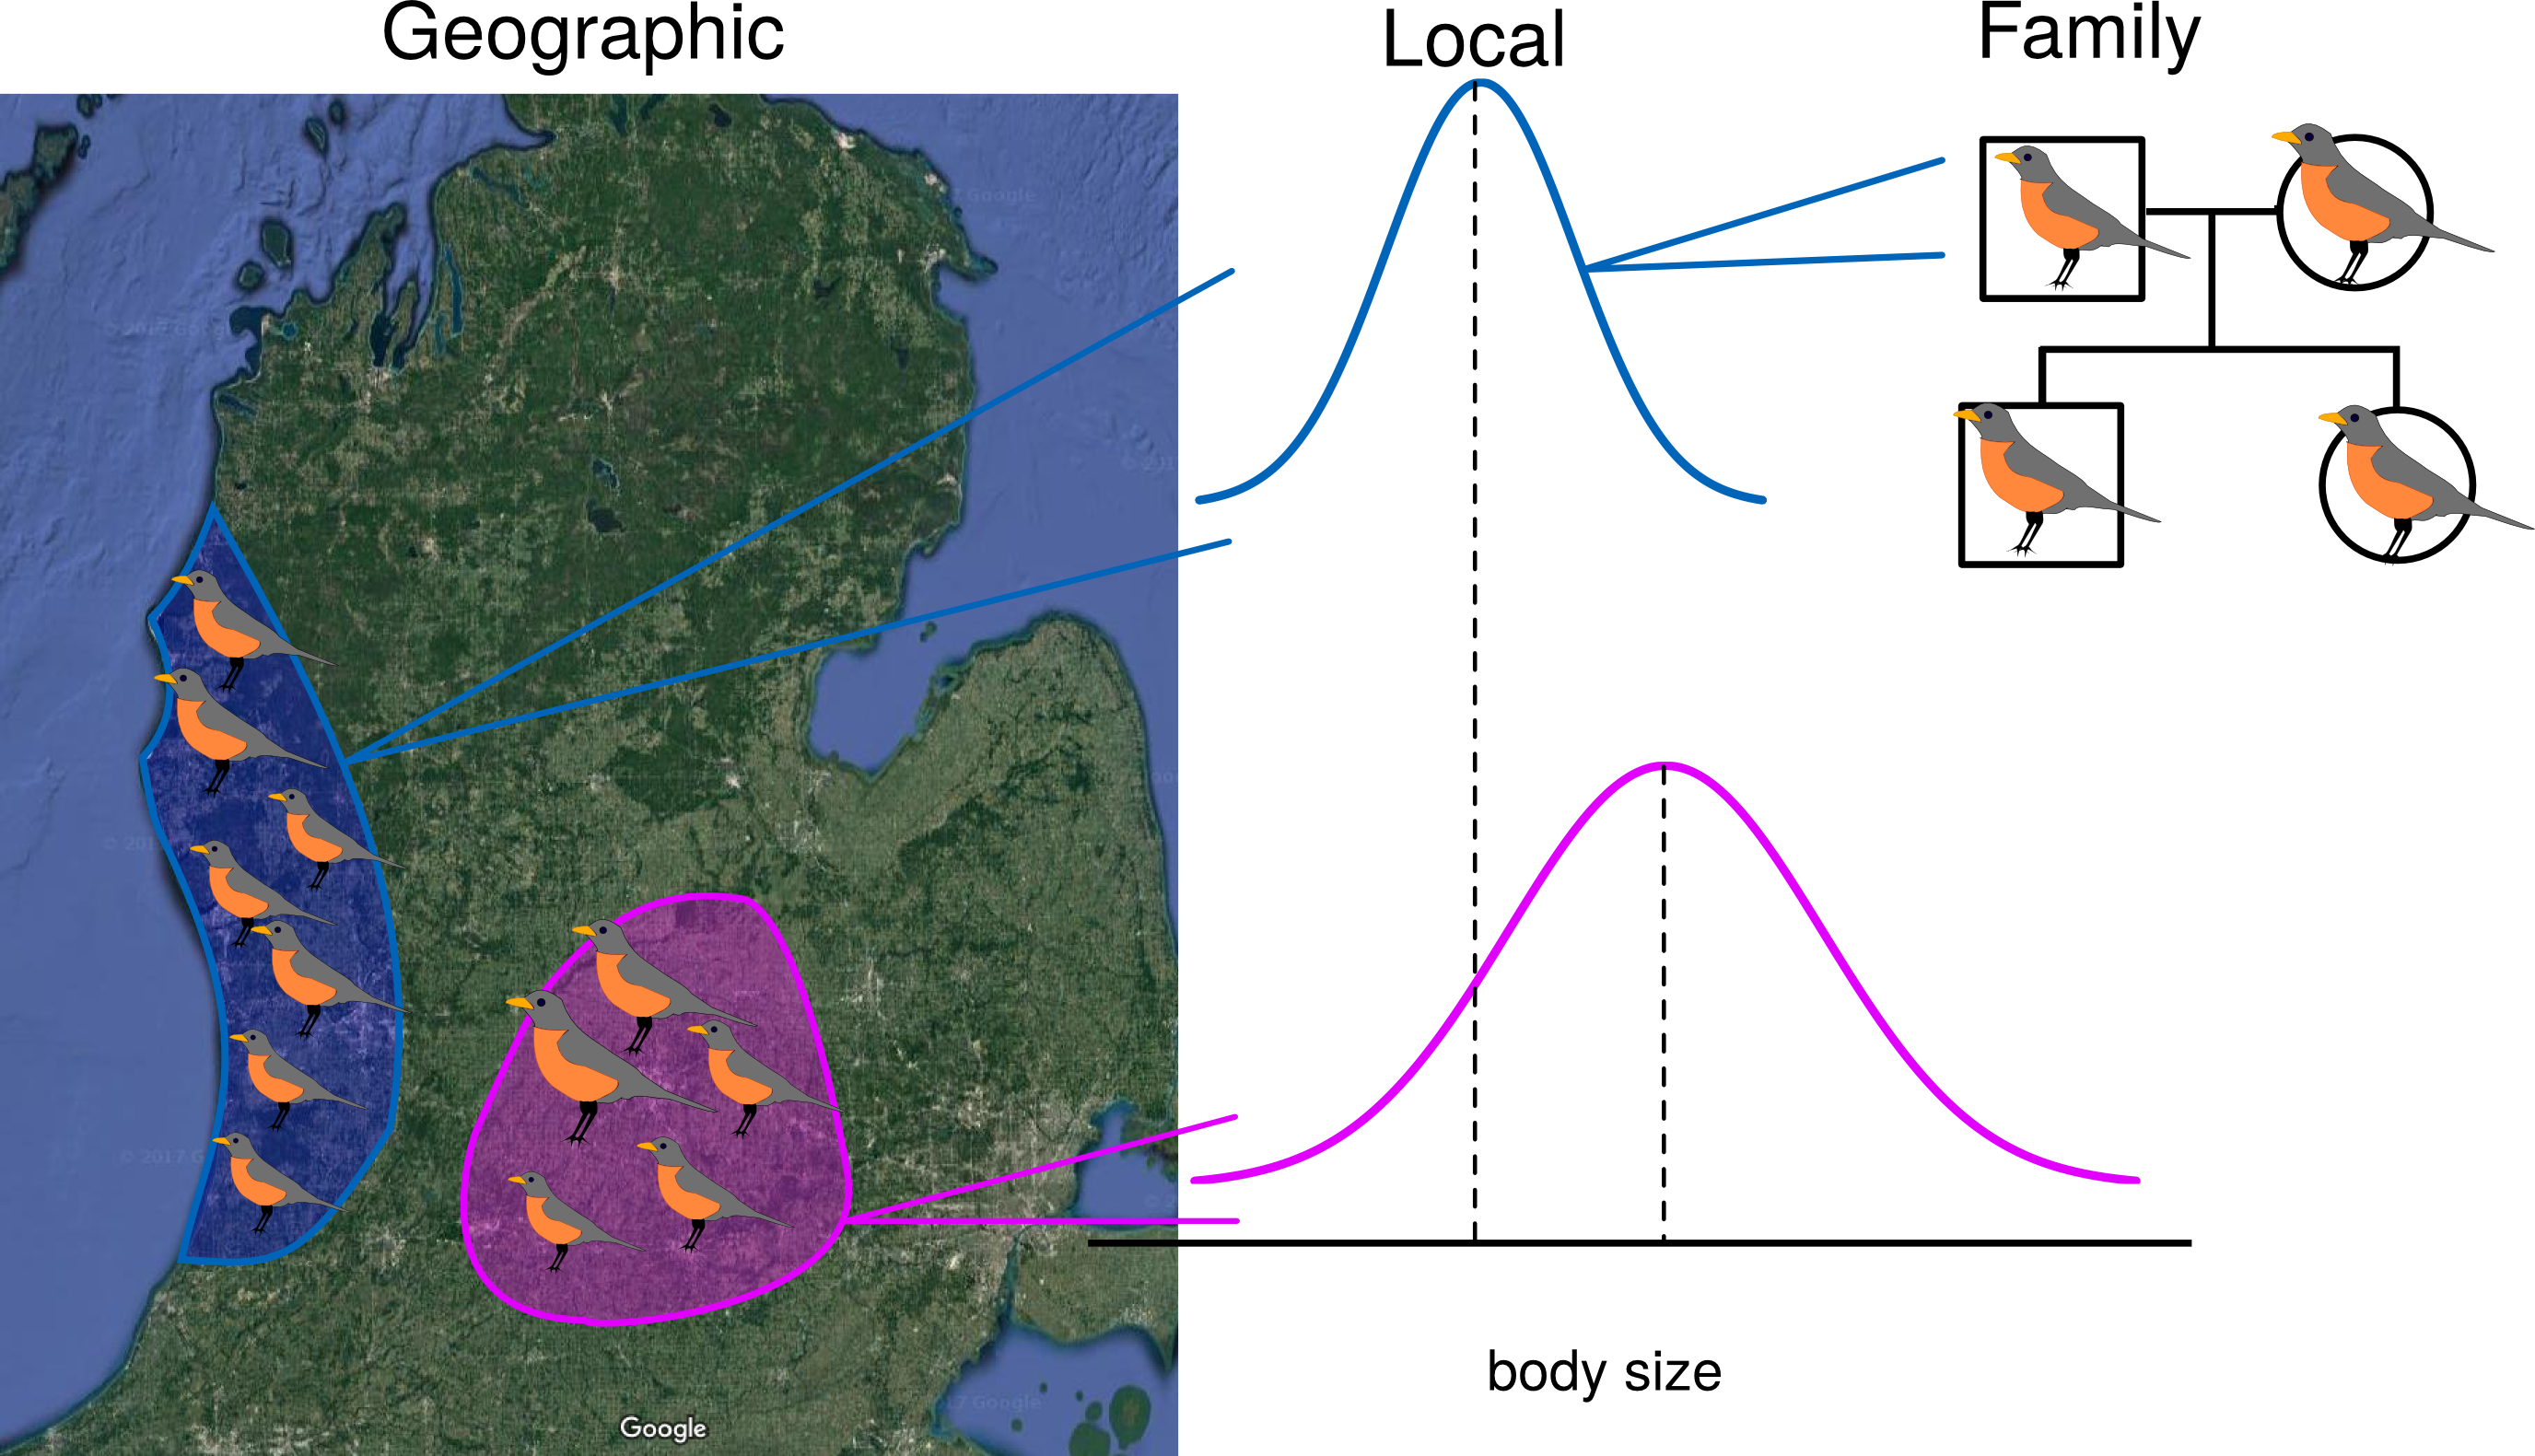
\includegraphics[width=\textwidth]{michigan_bird.png}
  \end{center}
\end{frame}

\begin{frame}{The factors affecting trait distributions}
  \framesubtitle{Genetic architecture}
  \begin{center}
    \includegraphics[width=\textwidth]{gene_arch.pdf}
  \end{center}
\end{frame}

\begin{frame}{The factors affecting trait distributions}
  \framesubtitle{Selection}
  \begin{center}
    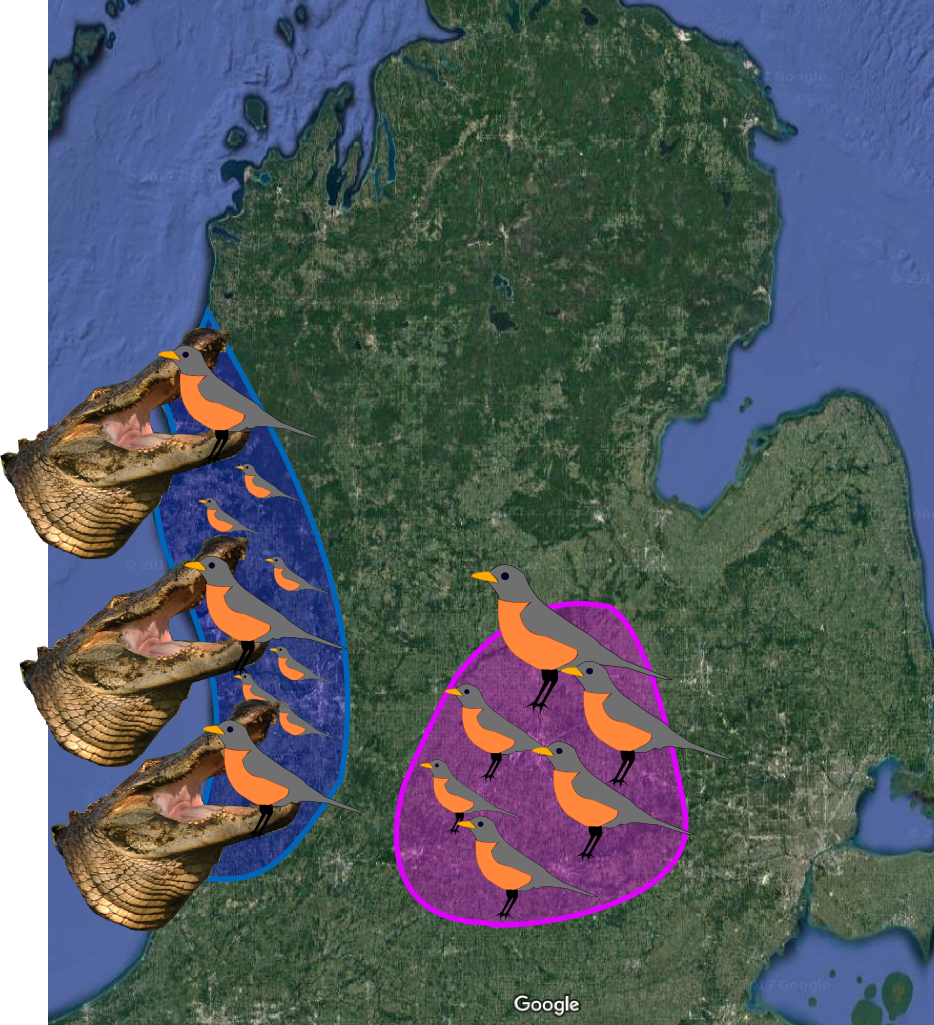
\includegraphics[width=0.5\textwidth]{michigan_gator.pdf}
  \end{center}
\end{frame}

\begin{frame}{The factors affecting trait distributions}
  \begin{block}{Population structure and demography}
    \begin{itemize}
    \item Geographic separation
    \item Local population size
    \item Breeding structure within families
    \end{itemize}
  \end{block}
  \begin{block}{Genetic architecture}
    \begin{itemize}
    \item Number of loci potentially affecting a trait
    \item Distribution of mutational effects
    \end{itemize}
  \end{block}
  \begin{block}{Selection}
    \begin{itemize}
    \item Local adaptation
    \item Stabilizing selection
    \end{itemize}
  \end{block}
\end{frame}

\begin{frame}{The factors affecting trait distributions}
  \begin{block}{Population structure and demography}
    \begin{itemize}
    \item Geographic separation
    \item Local population size
    \item Breeding structure within families
    \end{itemize}
  \end{block}
  \begin{block}{Genetic architecture}
    \begin{itemize}
    \item Number of loci potentially affecting a trait
    \item Distribution of mutational effects
    \end{itemize}
  \end{block}
  \begin{block}{\sout{Selection}}
    \begin{itemize}
    \item \sout{Local adaptation}
    \item \sout{Stabilizing selection}
    \end{itemize}
  \end{block}
\end{frame}

\begin{frame}{Models of neutral trait evolution}
  \begin{itemize}
  \item Serve as null models for goodness of fit tests
  \item Investigate the effects of demography and population structure in
    isolation
  \end{itemize}
\end{frame}

\begin{frame}{Models of neutral trait evolution}
  \begin{columns}
    \begin{column}{0.48\columnwidth}
      \begin{block}{Change driven by new mutations}
        \includegraphics[width=\columnwidth]{long_div.pdf}
      \end{block}
    \end{column}
    \begin{column}{0.48\columnwidth}
      \begin{itemize}
      \item $\sigma_m^2$: Mutational variance per generation
      \item {\footnotesize$Y_1 - Y_2 \sim N(0,2 t \sigma_m^2)$}
      \item  \footnotesize Lande (1976)
      \end{itemize}
    \end{column}
  \end{columns}  
\end{frame}

\begin{frame}{Models of neutral trait evolution}
  \begin{columns}
    \begin{column}{0.48\columnwidth}
      \begin{block}{Change driven by allele frequency divergence}
        \includegraphics[width=0.8\columnwidth]{short_div.pdf}
      \end{block}
    \end{column}
    \begin{column}{0.48\columnwidth}
      \begin{itemize}
        \item $Y_A$: Mean $t$ gen. ago
        \item $\sigma_A^2$: Variance $t$ gen. ago
        \item $f_{ij}$: Coancestry coefficient
        \item {\footnotesize$(Y_1,Y_2) \sim N(Y_A,
          \begin{pmatrix}
            f_{11} & f_{12}\\
            f_{12} & f_{22}
          \end{pmatrix}\sigma_A^2)$}
        \item \footnotesize Wright (1951)
        \end{itemize}
    \end{column}
  \end{columns}  
\end{frame}

\begin{frame}{Looking for adaptive differentiation among populations}
  \framesubtitle{The $Q_{ST}$ paradigm}
  \begin{block}{Does $Q_{ST}$ exceed a neutral expectation?}
    \begin{equation*}
    Q_{ST} = \frac{V_{\mbox{among populations}}}{V_{total}}
    \end{equation*}
  \end{block}
\end{frame}

\begin{frame}{Looking for adaptive differentiation among populations}
  \framesubtitle{The $Q_{ST}$ paradigm}
  Recent variations on this theme:
  \begin{itemize}
  \item Use GWAS hits to calculate genetic values and test for overdispersion
    (Berg and Coop, 2014)
  \item Full model of breeding experiments, population structure, and trait
    covariance (Ovaskainen et al., 2011)
  \end{itemize}
  \begin{figure}
    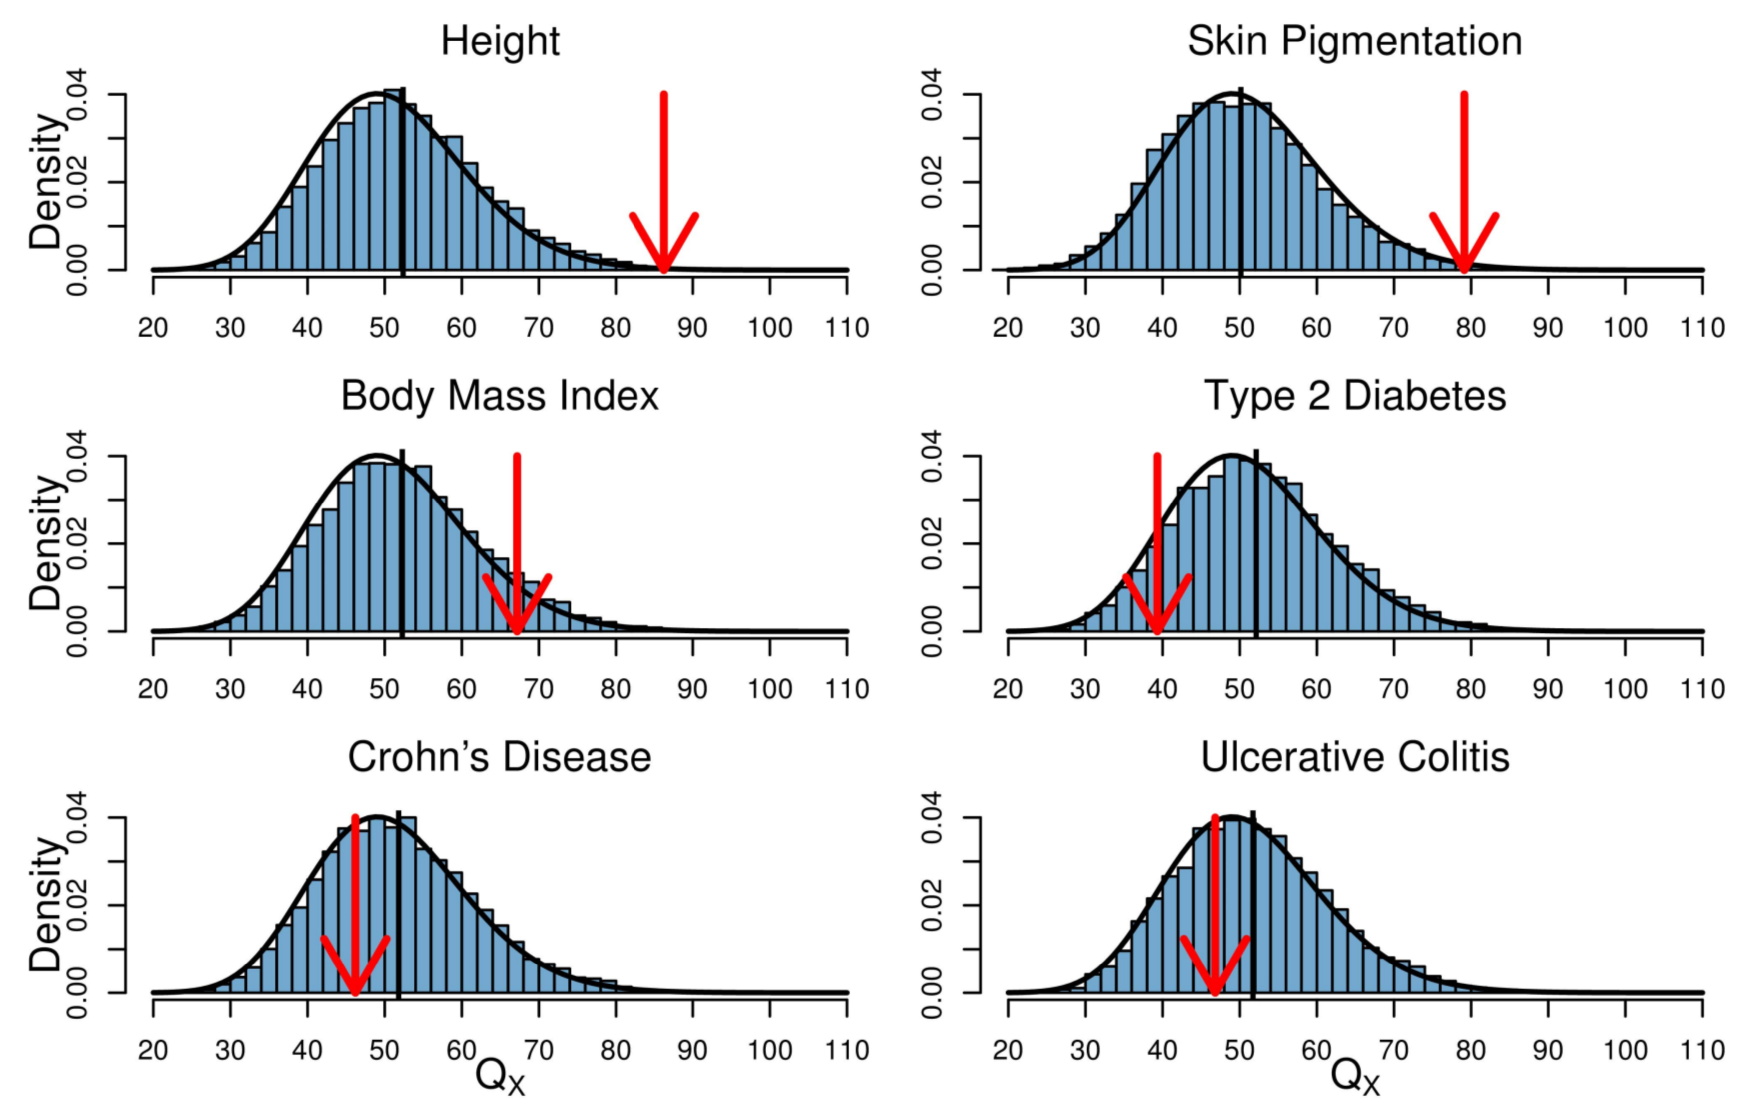
\includegraphics[width=0.6\textwidth]{berg_coop.png}
  \end{figure}
\end{frame}

\begin{frame}{A general neutral model should be based on the coalescent}
  \begin{itemize}
  \item Arbitrary population structure at arbitrary time scales
  \item Includes genetic architecture and the mutational distribution
  \end{itemize}
\end{frame}

\begin{frame}{Coalescent-based quantitative genetic models}
  \framesubtitle{That I've found so far $\ldots$}
  \begin{block}{Whitlock, 1999}
    Used coalescent argument to demonstrate that $\E[Q_{ST}]=\E[F_{ST}]$. 
  \end{block}
  \begin{block}{Griswold et al., 2007}
    Investigated the effects of shared ancestry and linkage disequilibrium on
    the genetic covariance matrix. 
  \end{block}
  %% \begin{block}{Schraiber and Landis, 2015}
  %%   Use a coalescent model to show that the normality assumption can be violated
  %%   when
  %%   \begin{itemize}
  %%   \item The number of loci affecting a trait is small.
  %%   \item Mutational distributions are skewed or fat-tailed.
  %%   \end{itemize}
  %% \end{block}
\end{frame}

\begin{frame}{Coalescent-based quantitative genetic models}
  \framesubtitle{Schraiber and Landis, 2015}
  \begin{columns}
    \begin{column}{0.55\columnwidth}
      \begin{center}
        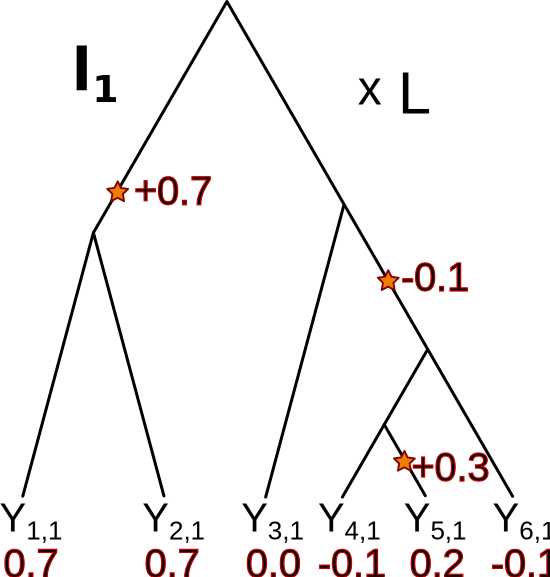
\includegraphics[width=0.9\columnwidth]{sl_model.pdf}
      \end{center}
    \end{column}
    \begin{column}{0.42\columnwidth}
      \begin{block}{Individual trait values}
        \begin{equation*}
          Y_i = \sum_{\ell=1}^L Y_{i,\ell}
        \end{equation*}
      \end{block}
      \begin{itemize}
      \item Sample size: $n$
      \item Mutation rate: $\T$
      \item Genealogies and mutational effects are both random variables.
      \item Additive mutational effects within loci (Kimura, 1965).
      \end{itemize}
    \end{column}
  \end{columns}
\end{frame}

\begin{frame}{Coalescent-based quantitative genetic models}
  \framesubtitle{Schraiber and Landis, 2015}
  \begin{block}{Conclusions}
    The normality assumption can be violated when
    \begin{itemize}
    \item The number of loci affecting a trait is small.
    \item Mutational distributions are skewed or fat-tailed.
    \end{itemize}
  \end{block}
\end{frame}

\begin{frame}{Goals}
  \begin{itemize}
  \item Extend Schraiber and Landis (2015) model to arbitrary genealogical
    distributions.
  \item How does the genealogical distribution influence deviations from
    normality?
  \item How do classic results fit into the coalescent framework?
  \end{itemize}
\end{frame}

\begin{frame}{The moment generating function for trait values}
  The moment generating function (mgf) for a sample of trait values is 
  \begin{definition}[Moment generating function]
    \begin{equation*}
      \varphi_{\mathbf{Y}}(\mathbf{k}) = \E\left[ e^{\mathbf{k} \cdot \mathbf{Y}} \right] =
      \int e^{\mathbf{k} \cdot \mathbf{Y}} \Pro(\mathbf{Y}=\mathbf{y}) \mbox{d}\mathbf{y}
    \end{equation*}
  \end{definition}
  \begin{itemize}
  \item $\mathbf{Y}$: vector of trait values (e.g. $\mathbf{Y} = (Y_a, Y_b, Y_c)$)
  \item $\mathbf{k}$: vector of dummy variables (e.g. $\mathbf{k} = (k_a, k_b, k_c)$)
  \end{itemize}
  \begin{block}{Usefulness}
    \begin{itemize}
    \item Calculating moments
    \item Deriving limiting distributions
    \end{itemize}
  \end{block}
\end{frame}

\begin{frame}{Genealogies also have generating functions}
  \framesubtitle{Lohse, Harrison, and Barton, 2011}
  \begin{block}{The genealogical mgf}
    \begin{equation*}
      \varphi_{\mathbf{T}}(\mathbf{s}) = \E\left[ e^{\mathbf{s} \cdot \mathbf{T}} \right] =
      \int e^{\mathbf{s} \cdot \mathbf{T}} \Pro(\mathbf{T}=\mathbf{t}) \mbox{d}\mathbf{t}
    \end{equation*}
  \end{block}
  \begin{itemize}
  \item $\mathbf{T}$: vector of internal branches (e.g. $\mathbf{T} = (T_a, T_b, T_c, T_{ab}, T_{ac}, T_{bc})$)
  \item $\mathbf{s}$: vector of dummy variables (e.g. $\mathbf{s} = (s_a, s_b, s_c, s_{ab}, s_{ac}, s_{bc})$)
  \end{itemize}
  \begin{figure}
    \includegraphics[width=0.5\textwidth]{topo.pdf}        
  \end{figure}
\end{frame}

\begin{frame}{Genealogical mgfs}
  Lohse, Harrison, and Barton (2015) derive the genealogy mgf, $\varphi_{\mathbf{T}}(\mathbf{s})$, for:
  \begin{itemize}
  \item Populations connected by migration
  \item The IM model 
  \item Step changes in population size
  \item Recombination between loci
  \end{itemize}
\end{frame}

\begin{frame}
  \begin{columns}
    \begin{column}{0.5\textwidth}
      \begin{center}
        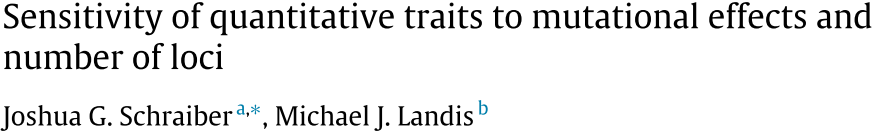
\includegraphics[width=\columnwidth]{schraiber_title.png}\\
        \vspace{.5cm}
        {\Large $\varphi_{\mathbf{Y}}(\mathbf{k})$}
      \end{center}
    \end{column}
    \begin{column}{0.5\textwidth}
      \begin{center}
        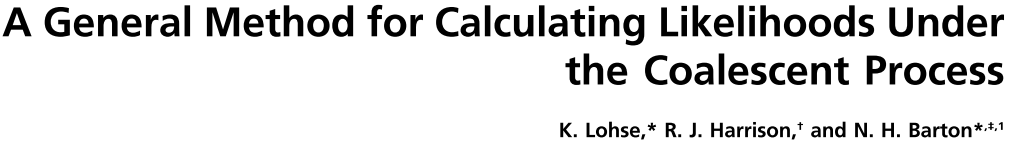
\includegraphics[width=\columnwidth]{lohse_title.png}\\
        \vspace{.5cm}
        {\Large$\varphi_{\mathbf{T}}(\mathbf{s})$}
      \end{center}
    \end{column}
  \end{columns}
  \begin{center}
    \includegraphics[width=0.5\textwidth]{arrows.pdf} \\
    {\Large ???}
  \end{center}
\end{frame}

\begin{frame}{Condition on the genealogy}
  \begin{center}
    \includegraphics[width=\textwidth]{tree_break.pdf}
  \end{center}
\end{frame}

\begin{frame}{Trait change is a compound Poisson process along each branch}
  \begin{columns}
    \begin{column}{0.5\textwidth}
      \includegraphics[width=\columnwidth]{compound_pois.pdf}
    \end{column}
    \begin{column}{0.5\textwidth}
      \begin{itemize}
      \item $\T \times t_{ab}$: expected number of mutations on the branch
      \item $\psi$: generating function of the effect size distribution
      \end{itemize}
    \end{column}
  \end{columns}
\end{frame}

\begin{frame}{The genealogy and trait mgfs are closely related}

  {\Huge
  \begin{equation*}
     \varphi_{\mathbf{T}}(\mathbf{s}) \longrightarrow \varphi_{\mathbf{Y}}(\mathbf{k})
  \end{equation*}
  \begin{equation*}
    s_{ab} \longrightarrow \T \left(\psi\left( k_a + k_b\right) - 1 \right)
  \end{equation*}
  }
  \begin{block}{A simple substitution}
    \Large
    \begin{equation*}
      \varphi_{\mathbf{Y}}(\mathbf{k}) = \varphi_{\mathbf{T}}(\mathbf{s})\Bigr|_{s_{\omega}=\frac{\theta}{2} \left( \psi\left(\sum_{a \in \omega}k_{a}\right) -1 \right)}
    \end{equation*}
  \end{block}
\end{frame}

\begin{frame}{Population model details disappear when the mutation rate is low}
  \begin{figure}
    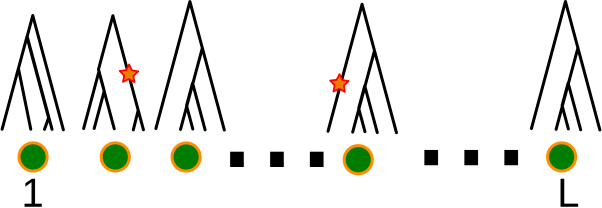
\includegraphics[width=\textwidth]{low_mut.pdf}        
  \end{figure}
\end{frame}

\begin{frame}{Only expected internal branch lengths matter}
  \begin{figure}
    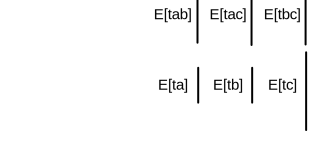
\includegraphics[width=0.5\textwidth]{tree_exp.pdf}        
  \end{figure}
\end{frame}

\begin{frame}{Infinitesimal limit: many loci, mutations of small effect}
  \begin{figure}
    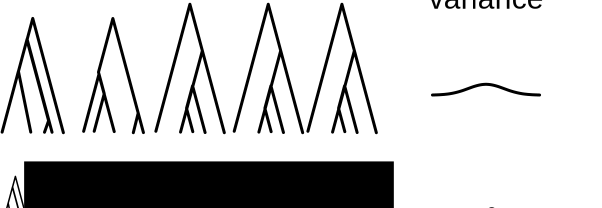
\includegraphics[width=0.7\textwidth]{infinitesimal.pdf}    
  \end{figure}
\end{frame}

\begin{frame}{Infinitesimal limit: a very simple result}
  \begin{columns}
    \begin{column}{0.5\textwidth}
      \begin{center}
        \includegraphics[width=\columnwidth]{coal_scheme.pdf}
      \end{center}
    \end{column}
    \begin{column}{0.5\textwidth}
      Normal distribution with:
      \begin{itemize}
      \item $\E[Y_a] = \E[T_{MRCA}] \mu$
      \item $\Var[Y_a] = \E[T_{MRCA}]\sigma^2$
      \item $\Cov[Y_a,Y_b] = (\E[T_{MRCA}] - \E[T_{a+b}]) \sigma^2$
      \end{itemize}
    \end{column}
  \end{columns}
\end{frame}

\begin{frame}{An example moment calculation: Kurtosis}
  \begin{definition}[Kurtosis]
    \begin{equation*}
      \mbox{Kurt}[X]=\frac{\E[(X-\E[X])^4]}{\Var[X]^2}.
    \end{equation*}
  \end{definition}
  \begin{figure}
    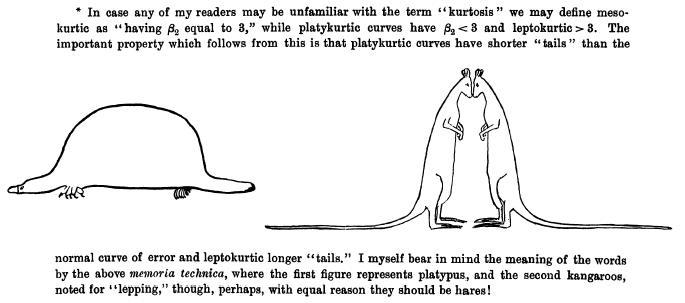
\includegraphics[width=\textwidth]{kurtosis-Student1927.png}        
  \end{figure}
\end{frame}

\begin{frame}{An example moment calculation: Kurtosis}
  \begin{block}{Expected population kurtosis}
    \begin{equation*}
      \E[\mbox{Kurt}] \approx 3 + \frac{\kappa}{L \T \E[T_2]}\left( \frac{4\E[T_2] - 6\E[T_3] +
        3\E[T_4]}{\E[T_2]}\right)
    \end{equation*}
  \end{block}
  \begin{itemize}
  \item $\kappa$: kurtosis of the mutational distribution
  \item $\E[T_i]$ expected $T_{MRCA}$ for a sample of size $i$. 
  \end{itemize}
  \begin{block}{Constant-size population}
    \begin{equation*}
      3 + \frac{\kappa}{2L\T \E[T_2]}
    \end{equation*}
  \end{block}
\end{frame}

\begin{frame}{An example moment calculation: Kurtosis}
  \begin{center}
    \includegraphics[width=0.5\textwidth]{foo.pdf}
  \end{center}
\end{frame}

%% \begin{frame}{Relationship with previously used normal models}
%%   \framesubtitle{Deep divergence}
%%   \begin{figure}
%%     \includegraphics[width=0.4\columnwidth]{long_div.pdf}      
%%   \end{figure}
%%   \begin{equation*}
%%     \footnotesize
%%     (Y_1 , Y_2) \sim N(\E[T_{MRCA}] \mu \mathbf{1}, \sigma^2
%%     \begin{pmatrix}
%%       \E[T_{MRCA}] & (\E[T_{MRCA}] - \E[T_{1,2}])  \\
%%       (\E[T_{MRCA}] - \E[T_{1,2}]) & \E[T_{MRCA}]
%%     \end{pmatrix})
%%   \end{equation*}
%%   \begin{equation*}
%%     Y_1 - Y_2 \sim N(0, 2 \sigma^2 \E[T_{1,2}])
%%   \end{equation*}
%%   \begin{equation*}
%%     E[T_{1,2}] \approx t
%%   \end{equation*}
%% \end{frame}

%% \begin{frame}{Relationship with previously used normal models}
%%   \framesubtitle{Recent divergence}
%%   \begin{columns}
%%     \begin{column}{0.5\textwidth}
%%       \begin{figure}
%%         \includegraphics[width=\columnwidth]{short_div.pdf}   
%%       \end{figure}
%%     \end{column}
%%     \begin{column}{0.47\textwidth}
%%       \begin{equation*}
%%         (Y_1,Y_2) \sim N(Y_A,
%%           \begin{pmatrix}
%%             f_{11} & f_{12}\\
%%             f_{12} & f_{22}
%%           \end{pmatrix}\sigma_A^2)
%%       \end{equation*}
%%     \end{column}
%%   \end{columns}
%% \end{frame}

\begin{frame}{Conclusions}
  \begin{itemize}
  \item We can investigate the sampling distribution of trait values by first
    deriving or looking up the mgf for the genealogy.
  \item This is simplified considerably by only allowing one mutation per locus.
  \item Deviations from normality will depend on demography and population
    structure.
  \end{itemize}
\end{frame}

\begin{frame}{Future directions}
  \begin{itemize}
  \item Incorporate recombination
  \item Connect neutral models for trait evolution at different levels of
    divergence.
  \end{itemize}
\end{frame}

\begin{frame}{Acknowledgments}
  \begin{itemize}
  \item Funding: NSF GRFP
  \item Novembre lab members
  \item Midwest popgen conference organizers
  \end{itemize}
\end{frame}

\end{document}
